\section{Introduction}
In this chapter we consider similar projects that have been done and how they relate to the project development and execution in relation to our project. We also look at their shortcomings and how they're addressed in our solution.


\section{Ubiquitous Computing approaches}
The domain of ubiquitous computing according to Michael Friedewalda and Oliver Raabe is concerned with countless small, wirelessly intercommunicating microprocessors, embedded into objects. Such techniques are applied in similar concepts, such as ``the Internet of things''.The main motive in these domains is assisting people and optimizing economic and social processes through the use of microprocessors and sensors.

\begin{figure}[h]
    \begin{center}
        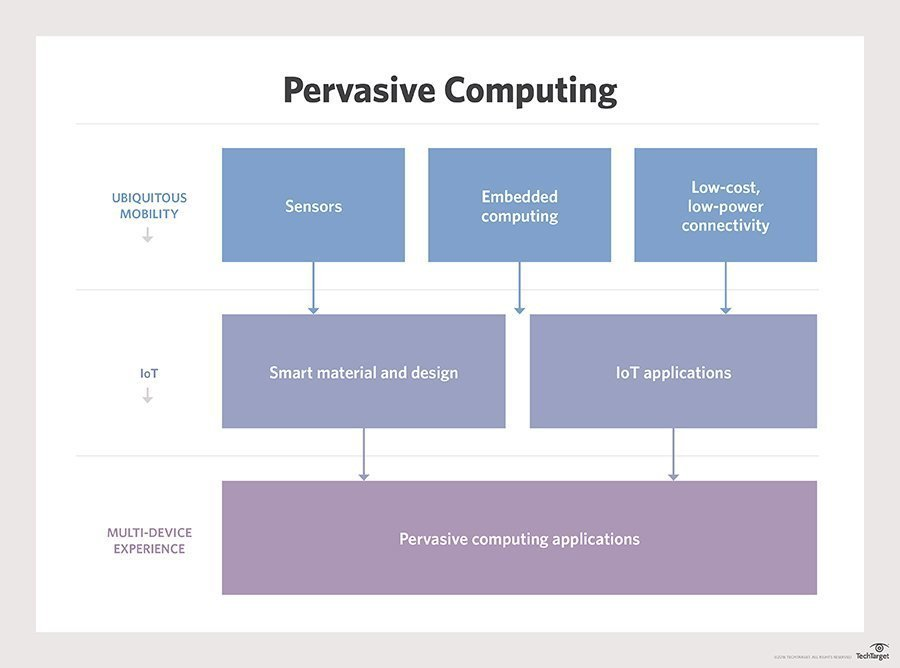
\includegraphics[scale = 0.34]{images/ubq}
        \caption{A sketch of a ubiquitous computing application}
    \end{center}
\end{figure}
These microprocessors are equipped with sensors enabling them to capture information about their current environment or process information and communicate over a network with other similar devices\cite{friedewald_ubiquitous_2011}.

Ubiquitous computing systems consist of features such as:\cite{friedewald_ubiquitous_2011}
\begin{itemize}
    \item The system is decentralised
    \item Computers are embedded in other devices
    \item Real-time information is readily available for users
    \item The system is able to adapt basing on current information.
\end{itemize}

This concept has a number of real world applications in domains such as retail, industrial production, health care and this is achieved through implementations such as tracking applications, wearable devices like smartwatches.

In this section looks at projects that have been done in the area of ubiquitous computing with an aim of addressing a challenge similar to ours. We also look at their shortcomings and how they're addressed in our project.

\subsection{Use of RFID sensors}
One approach that's based ubiquitous computing techniques is the use of an RFID system. This system has two main components:
\begin{itemize}
    \item A transponder: This is the tag that holds information, found on the object to be identified
    \item A reader/interrogator: This device is able to capture data from the tag.It has a radio frequency module,  control unit and coupling element for linking to the transponder. Additionally, an interface is added to pass on data captured from the transponder to a different system
\end{itemize}
\begin{figure}
    \begin{center}[h]
        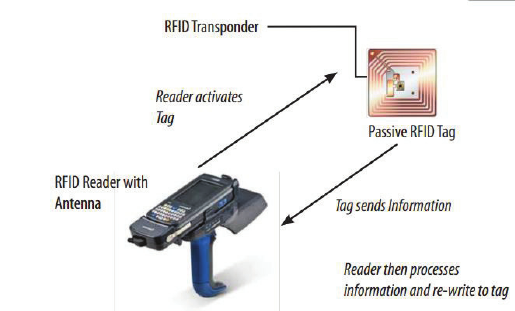
\includegraphics[scale = 0.3]{images/rfid-pic}
        \caption{Components of an RFID system}
    \end{center}
\end{figure}
Sabbir Ahmed et al. in 2019 also proposed a similar solution.Their proposed system would simplify toll payment through use of RFID tags placed on digitised license plates of all vehicles.Once the tag is scanned, and the motorist has a sufficient balance on their account, the vehicle is granted access\cite{ahmed_automated_2019}.


Another study by Etqad Khan et al. in 2018 proposed a system similar to ours that would ease payment of toll fees using RFID tag that would be linked to motorists' personal accounts where would have a mobile e-wallet on which a given amount would be saved.The system also provides a mobile application to view their past payments\cite{khan_automated_2018}.

\subsubsection{Research Gap}
These two identified studies are constrained in our project scope\’s context, because:
\begin{itemize}
    \item Implementing such solutions would first off require digitisation of all vehicle license plate, an endeavour that has not yet been taken on by the government of Uganda.
    \item Long range RFID tags and scanners are costly to purchase which would be needed in this use case are costly ,and would thus the need for a low-cost solution that is also widely accessible such as via mobile.
\end{itemize}



\clearpage

\subsection{Use of GPS Software and Cell Towers}
Research on how this can be leveraged in easing toll & parking fee payment has been done by others. In 2020, Danang Dismantoro, Istas Pratomo and Surya Sumpeno also proposed a mobile application that allowed payment of these fees via GPS software\cite{el-rabbany_introduction_2002,dismantoro_minimizing_2020}. The system was tested through simulations in Vissim software \cite{ptv_vissim_traffic_2022}, which they believe was able to simulate the real world condition at tollgates. Cell phone towers and GPS technology are used to identify the motorist’ s location and if the motorist happens to be within the toll’s gate vicinity, the money is automatically deducted from their personal account.

\subsubsection{Research Gaps}
\begin{itemize}
    \item No physical implementation of this system was realised
    \item The researchers acknowledge the need for a deeper feasibility study and the fact as it has some shortcomings.
    \item Some scenarios are unaccounted for such as if one is near a cell tower but does not necessarily intend to access the tollgate,they’ll have their money deducted even without actually using the gate.
\end{itemize}

\clearpage


\section{Mobile Applications}
In this section we discuss some of the mobile applications that have been developed to address the challenge of parking in urban areas. We also look at their shortcomings and how they're addressed in our project.

\subsection{ParkMobile}
Parkmobile is a leading mobile application launched in 2009 in the United States of America that allows motorists to find and pay for parking on their phone. This application is currently used in approximately used in three thousand locations in North America, and also has garnered over 43 million users processing over 113 million parking transactions in 2022.

It offers various features and benefits for its users, such as making prepayments and reserving parking points at any given location. It also offers a rewards program that allows users to earn points for every parking transaction and redeem them for discounts or free parking. Parkmobile also supports Google and Apple Pay for a faster and more secure payment process. \cite{ParkMobile2023}
The project has had good traction since it was launched and in 2022 it generated 9.1 million dollars in revenue , with an average revenue per employee of 52,906 dollars. Parkmobile was acquired by EasyPark Group, a Swedish company that provides smart parking and mobility solutions, in June 2021.

\subsection{FlowBird}
The Flowbird parking app is a cloud-based platform developed in France that allows users to pay for parking in three simple steps and access different parking solutions to meet their personal needs. It offers similar features to the ParkMobile application previously discussed such as mobile-based payments, statistics of available parking places, etc\cite{Flowbird2023}.

\subsection{Research Gap}
The main shortcoming of these applications is the fact that they were built and are currently only used in developed countries. As of this writing there exists no equivalent mobile application to enable parking and toll fee payments in Uganda. This is the gap that our project aims to address.

\clearpage


\section{Makerere University Automated Payment System}
This is the existing system in place and was the main case study of our research. The project was commenced in 2014 by Makerere University in collaboration with Kenya Airport Parking Services\cite{wamai_mak_2014} .
From our interviews with Mr. Twinomusinguzi Julius, the current manager of the existing system we learned that the system costs approximately 1.5 billion shillings to set up. It consists of a ticketing machine that issues tickets to motorists, as well as various payment points where payments are made and human labour to receive money, give change and manage the systems in case of breakdown. Some of the challenges in this system include:

\begin{itemize}
    \item Frequent malfunction of the ticketing machines. This occurs due to their wear and tear over time. As previously mentioned, this equipment is costly not just to purchase but maintain as well.
    \item Fraud by the system employees. A common way this occurs is when a motorist instead of paying at the point, they're granted access by the gate attendants, who then retain the money for themselves. From our interviews, we also determined that students who are exempt from paying the parking fees upon proving their status, sometimes pay the gate attendants to be granted access in case they don't have their student IDs with them. This can be addressed by having a system that automatically detects students and grants them access without the need for human intervention.
    \item Difficulty in locating a payment point for motorists. The university is large about 300 acres with payment points placed at different points around it. For people visiting the area for the first time, locating these points can be a challenge thus the need for a more convenient way of making payments.
    \item Hefty fines for lost tickets as motorists who misplace their tickets are required to pay a fine of 50,000 Uganda Shillings. From our interviews we were informed that a high fee was set because with a lower fee, some motorists park for long periods and intentionally lose their tickets to pay a fine that's lower than their actual parking bill.
\end{itemize}

\clearpage

\section{Uganda National Roads Authority Express Highway}
\begin{figure}[h]
    \begin{center}
        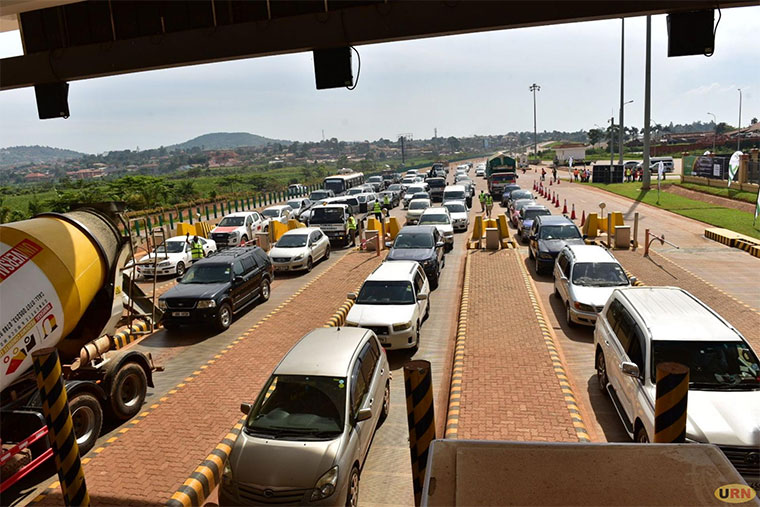
\includegraphics[scale = 0.3]{images/ebbs}
        \caption{Toll gate at Kampala Entebbe Express Highway}
    \end{center}
\end{figure}
The Uganda National Roads Authority in 2022 launched the Kampala Entebbe Express Highway, a Ugandan government project worth approximately 450 million dollars developed to help ease transport flow in Kampala city. Access to the highway is via the tollgates where motorists can make both cash and digital cashless payments. For cashless payments, motorists use an UPESI card.\cite{unra_news_2022}. A motorist purchases an UPESI card that they then load a given amount of money and upon arrival at the tollgate, they swipe the card. The fee is then deducted from the card and the motorist is then granted access.

The main gap with the approach is motorists often resort to only using the cash payments that result in delays and other issues because they find it easier than purchasing an UPESI card. Additionally, the process of loading money onto the card is unnecessarily long.

\clearpage

\section{Our Contribution}
Alot of work has been done by other researchers to address the issue of digital payments for toll / parking fees. Many of these solutions leverage RFID technology as an alternative to the physical cash payments.This would however require purchasing costly scanners and tags, thus the need for a similar but cheaper solution. Additionally, the existing mobile applications meant to help address this issue are only available in developed countries, and as of this writing, no system has been developed in Uganda.
The biggest benefits to our proposed system:
\begin{itemize}
    \item Designing and implementing a cross platform mobile applicaton and an embedded microcontroller that interact using QR codes to facilitate parking access and payment. The mobile app is developed using the Flutter framework guaranteeing its accesibility to various mobile platforms i.e Android, iOS. More details on this are discussed in the presentation of results section.
    \item Using low cost microcontrollers( ESP-32), we were able to program them with a camera module to be able to read and capture QR-code values, and interact with a server to verify motorists payments. This we believe is a cheaper alternative to use of RFID tags.
    \item Leveraging all local payment platforms e.g MTN mobile money, Airtel Money thus various providers are all catered for.
\end{itemize}
